\documentclass[11pt,titlepage]{article}
\usepackage{TCSToolkit}

\newcommand{\dofloor}[1]{\lfloor#1\rfloor}
\newcommand{\doceil}[1]{\lceil#1\rceil}

%%%%% Stuff you can change %%%%%%%%%%%%%%%%%%%%%%%%%%%%%%%%%%
\newcommand{\myname}{Lev Stambler}
%

%% Custom Commands
\newcommand{\rationalPeriod}{{T^j}'}
\newcommand{\rationalPeriodTotal}{{T}'}
\newcommand{\statePeriod}{T^j}
\newcommand{\rationalAngleJ}[2]{{\theta^{#2}_{#1}}}
\newcommand{\rationalAngle}[1]{{\theta^j_{#1}}}
\newcommand{\rationalAngleNotime}{{\theta}^j}
\newcommand{\state}[2]{{s_{#1}}^{#2}}
\newcommand{\stateNotime}[1]{s^{#1}}
\newcommand{\totalPeriod}{T}
\newcommand{\totalState}{\pmb{s}_i}
\newcommand{\totalStateNotime}{\pmb{s}}
\newcommand{\comb}{Comb}
\newcommand{\combWithState}[1]{Comb\left(s^1_{#1}, s^2_{#1}, ..., s^k_{#1}\right)}
\newcommand{\inclIndic}[2]{{\mathrm{incl}_{#1}^{#2}}}
\newcommand{\numbToAngle}{\frac{2\pi}{b^j}}
\newcommand{\numbToAngleNoJ}[1]{\frac{2\pi}{b^{#1}}}
\newcommand{\combSingleTermCos}[1]{\prod_{j=1}^k \cos\left(\numbToAngle \cdot \theta^j\right) ^ {\inclIndic{#1}{j}}}
\newcommand{\digSumPeriodic}{\sigma^j}
\newcommand{\digSumPeriodicNoJ}{{\sigma}}
\newcommand{\totalOverRationalFrac}{\frac{\totalPeriod}{\rationalPeriodTotal}}
\newcommand{\changeTotalOneDim}{\Delta P_{0, T}^d}
\newcommand{\digit}{\mathrm{digit}}
\newcommand{\commonBase}{{\pmb{b}}}
\newcommand{\numbToCommon}{\frac{\commonBase}{b^j}}
\newcommand{\commonToAngle}{\frac{2\pi}{\commonBase}}
\newcommand{\sinOrCos}{\phi^j}
\newcommand{\combSingleTerm}[1]{\prod_{j=1}^k \sinOrCos\left(\numbToAngle \cdot \theta^j\right) ^ {\inclIndic{#1}{j}}}


%
% Final tip: you can reference HW5 in your TeX using \Cref{hw:5}; 
% and, you can reference HW5.Problem3 in your TeX using \Cref{prob:5.3}
%


%%%%% Section-renaming code by egreg
\makeatletter
% we use \prefix@<level> only if it is defined
\renewcommand{\@seccntformat}[1]{%
  \ifcsname prefix@#1\endcsname
    \csname prefix@#1\endcsname
  \else
    \csname the#1\endcsname\quad
  \fi}
% Now we define our homework section prefixes
% \newcommand\prefix@section{Homework \thesection: }
% \newcommand{\prefix@subsection}{Problem \thesubsection: }
% \newcommand{\prefix@subsubsection}{Section \thesubsubsection: }
\makeatother
%%%%%




\begin{document}

\title{Drawing Math}

\author{\myname}

\date{\today}

\maketitle

\pagebreak
\section*{Abstract}
Given an object in cartesian space, we ask whether a repeating sequence 
of spherical updates to the object's position cause it to travel on a closed path.
A spherical update to a position in $D$-dimensional space can be written as
$\left(r, \theta_1, \theta_2, ..., \theta_{D-1}\right)$.
In this paper, we consider $D-1$ non-terminating
rational numbers where for time-step $i$, the spherical updates' difference function
is given by $r' \leftarrow r$, 
$\theta_1' \leftarrow \theta_1 + \mathrm{digit}(q_1, i)$, ..., 
$\theta_{D-1}' \leftarrow \theta_{D-1} + \mathrm{digit}(q_{D-1}, i)$.
We then proceed to derive a formula for finding if the object takes a closed, repeating path.
Moreover, we explore interesting properties of this problem and
relate it to discrete log, roots of a multinomial, and center of mass.



\section{Introduction}
A glum Pittsburgh day inspired the authors to take a random walk down YouTube's recommended
when they encountered the Numberphile video on ``Plotting Pi" \cite{NumberphileVid}.
In the video, Henderson and Brady introduce the idea of taking a Python Turtle and
deriving a series of updates to its position based off of various decimal sequences, 
some rational, some irrational. More specifically, they place an object in 2D, cartesian
space starting at $(0, 0)$ and ``facing" to the right. They then take a generating number, like $\pi$ or $35/99$, 
which gives a decimal sequence ($3.14...$ and $0.\bar{35}$ respectively). 
Then, at time step $i$, $i \geq 1$, they rotate the object by the $i$th digit divided by the base of
the decimal sequence. Then, the Turtle moves a constant distance in the direction which it faces.
For example, if the second digit is 4, the turtle is rotated by $\frac{4}{10}$ths of a circle
counterclockwise at time step 2 and then moves 10 units in its new direction.
% TODO: diagram, timestep 1 --> 2 --> 3

Whenever the Turtle moves, the program draws a red line along the Turtle's path. Thus,
different lines are drawn.
The authors noticed that using rational numbers to generate the sequence often drew geometrically
aesthetic, closed shapes.

\begin{figure}[ht]
  \centering
  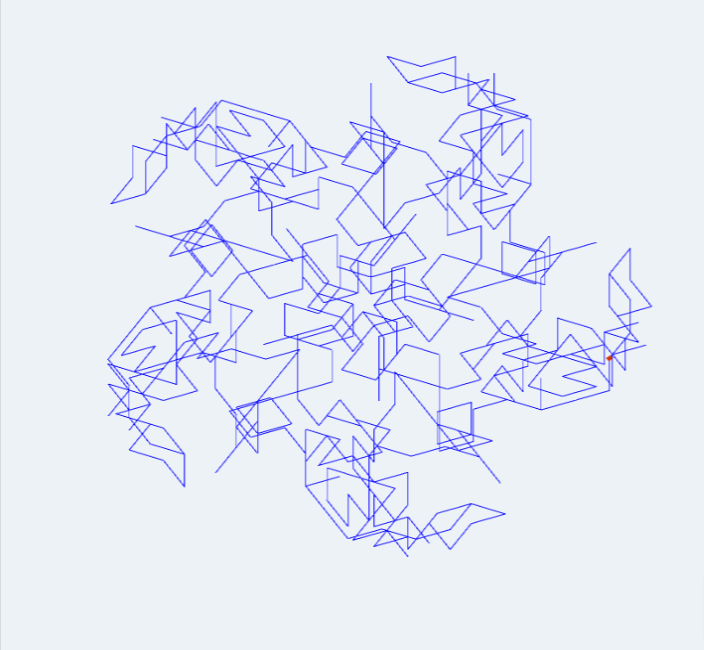
\includegraphics[width=8cm]{fig/Turtle1D13Div113.png}
  \caption{The closed shape generated from $\frac{13}{113} = 0.0977443609...$ in base $10$.}
\end{figure}
\begin{figure}[ht]
  \centering
  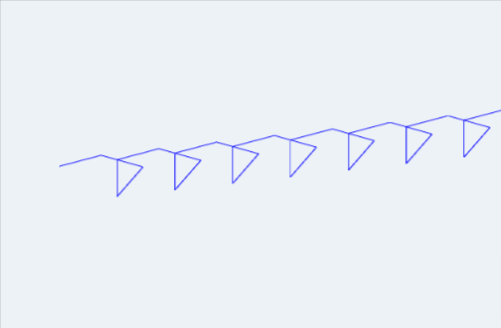
\includegraphics[width=8cm]{fig/Turtle1DNotClosed.png}
  \caption{A non-closing shape generated from $\frac{2134}{9999} = 0.\overline{2134}$ in base $10$.}
\end{figure}

Naturally, the authors were curious whether a Turtle in ``3D" would also draw 
aesthetic shapes. In other words, what if the Turtle's orientation was described
by 2 angles, pitch and yaw. The pitch and yaw would then by independently updated
by 2 decimal sequences generated from 2 rational numbers.
% TODO: figure
After writing the program, we noticed that the Turtle would often fail
to close. In other words, the Turtle would go off in one direction forever.
% TODO: picture of failing to close.
But, the Turtle \textit{sometimes} closed.

The authors then proceeded to ask why the Turtle would sometimes close and sometimes
go off into the ether. After finding a closed form solution in 3 dimensional space,
we proceeded to ask the same question in $D$ dimensional space: given $D - 1$ 
rational decimal sequences which determine the Turtle's orientation in space,
does the Turtle move in a closed shape (i.e.\ is the Turtle position always contained
within some $D$ dimensional sphere off constant radius)?

\section{Background}
- Digital math
- Euler's formula
- I payed attention in some of my lectures

\section{Definitions and questions}
\subsection{Definitions}
Say you (yes you!) had a turtle living in $D$ dimensional Euclidean
space and in discrete time. At time step $i$, where $i \in \Z$ and $i > 0$,
the turtle has position $p_i \in \R^D$.
Then, lets define $\Delta p_{i+1} = p_{i+1} - p_i$; in other words, $\Delta p_{i+1}$ is the change in position from time $i$ to $i + 1$.

Now say that the turtle's movement is determined by $k$ seed parameter drawn from
the same set. Then, for some state space $\mathcal{S}$,
define $s_i^j \in \mathcal{S}$ to be some arbitrary
state associated with timestamp $i$ for the $j$th seed parameter where $j \in [k]$.
Also, define $\pmb{s}_i = (s_i^1, s_i^2, ..., s_i^k)$.
Next we will define a set of functions $SU^j: \mathcal{S} \rightarrow \mathcal{S}$
(for $S$tate $U$pdater) such that $s_{i + 1}^j = SU^j(s_i^j, i)$. Note that for
$j, a \in [m]$ where $j \neq a$, $s_{i+1}^j$ is determined solely by $s_i^j$ and $i$ and not
$s_i^a$.

Now that we have our machinery built up, lets define $Comb: \mathcal{S}^k \rightarrow \R^d$ such that
$$
  \Delta p_{i + 1} = \combWithState{i + 1}.
$$
In other words, $Comb$ takes in the state of each seed and
returns an update to the position of the turtle.

Finally, let us define
$$
  \Delta P_{a, b} = \sum_{i = a}^{b} \Delta p_i.
$$
In other words, $\Delta P_{a, b}$ is the change in position from timestep $a$ to $b$.

\subsection{The problem}
Say we are given, $Comb$, hh$SU^j$, $p_0$, and $s^j_0$ for all $j \in [k]$.
Informally, the question is whether the turtle draws a ``closed" shape or not.\\
More formally, is there some period $T$ such that 
$$
  p_{i + \ell T} = p_{i}
$$
for $i, \ell \in \N$.
Then, note that if there exists a period $T$ such that 
$\Delta P_{i, i + \ell T} = 0$ for all $i, \ell \in N$, 
$p_{i + \ell T} = p_{i}$ and the turtle forms a closed shape.

\subsection{Specifying the task ahead of us}
For our case, we consider $Comb, SU_i^j$ to all be memoryless (i.e.\ there output
is uniquely determined by the current input). So, we can simplify the overall question.
If, $\pmb{s}_i = \pmb{s}_{i + \ell T}$ for some $T \in \N$ and all $i \in \N$, then 
$\Delta p_{i} = \Delta p_{i + \ell T}$. So then,
$\Delta P_{i, i + \ell T} = \Delta P_{i, i + \ell' T}$ for all $\ell, \ell' \in \N$.
Thus, $T$ is a period of the change in position. We can thus
break down our problem into two parts:
\begin{enumerate}
  \item Finding the period, $T$, of the state $\pmb{s}$.
  \item Checking whether $\Delta P_{i, i + T} = 0$.
\end{enumerate}

\subsection{Some more restrictions on our problem}
We further restrict the problem by only considering $\mathcal{S} = \N^4$ where for $(n, d, b, \theta) \in \mathcal{S}$,
$n$ is the numerator of a rational in fraction form, $d$ is the denominator, 
$b$ is the base (i.e.\ base 10, base 12, etc.),
and $\frac{2\theta}{b \pi}$ is an ``angle" associated with the state.

Then, let $\sinOrCos: \R \rightarrow \R$ equal $\cos$ or $\sin$. 

Now, we will only consider
$$
  SU_i^j(n, b, d, \theta) = (n, b, d, \theta + \mathrm{digit}(n, b, d, i) \mod b).
$$
where $\mathrm{digit}(n, b, d, i)$ gives us the $i$th digit of the decimal expansion of $\frac{n}{d}$
in base $b$. For the sake of convenience, we will use the word ``rational parameter" 
instead of ``seed parameter" from here on out.

Moreover, we consider the case where
$$
  Comb((., ., ., ., \theta^1), (., ., ., ., \theta^2), ..., (., ., ., ., \theta^k)) =
    \left(\combSingleTerm{1}, ..., \combSingleTerm{D}\right)
$$
where $\mathrm{incl}_d^j \in \set{0, 1}$ for $d \in [D]$ indicates whether to include a given
$x \in R$ determined by rational parameter $j$ for position update in the $d$th dimension.

Finally, for simplicity's sake, assume that $\theta = 0$ for all $(n, b, d, \theta) \in \pmb{s}_0$,
$n < d$, and $\frac{n}{d}$'s decimal expansion is periodic after some $N \geq 0$ decimal places
and does not terminate in base $b$.

Also, lets set 
$$\commonBase = \lcm{(n, b, d, \theta) \in \pmb{s}_0} b.$$
In other words,
$\commonBase$ can be thought of as a ``common base" among all rational parameters.

\subsubsection{Some intuition}
While the restrictions may seem arbitrary, they aptly match our original problem statement.
The original problem statement derives a spherical change in position based off of a rational number's
digit at a particular timestep. The polar change in position also has a fixed radius. Translating
from a polar to cartesian update then only requires products of $\sin$s and $\cos$s. See \cite{NDimSphericalCoord}
for more details.

Take the three dimensional case for instance. The turtle's update cartesian space
is given by 
\begin{align*}
  x &= \cos(\alpha)\\
  y &= \sin(\alpha) \cos(\beta)\\
  z &= \sin(\alpha) \sin(\beta)
\end{align*}
where $\alpha = \numbToAngleNoJ{1} \cdot \theta^1$ and 
$\beta = \numbToAngleNoJ{2} \cdot \theta^2$. We can thus see that our definition
of $\comb$ captures the three dimensional case.

% TODO: clear up.

% TODO: put your own diagram in!!


\section{Does it close?}
In understanding whether a set of given rationals, bases, and updated functions 
draw a closed shape in $D$ dimensional space, we first need to find the period of 
the update delta, $\Delta p_i$. We then know that the total update over a period will be repeated 
indefinitely. Consequently, we then seek to find the total change in position over a period. 
If the total change is $0$, the shape will close as the Turtle will end up at its starting point
after every period length. If the total update is nonzero, the Turtle will not draw a closed
shape.

\subsection{Finding period $T$}
We now show how to find a period $T$ of state $\pmb{s}$.

\subsubsection{Finding the period of a fraction}
For some $(n, b, d, \theta) \in \pmb{s}_0$,
we have that the period of the decimal expansion of $\frac{n}{d}$
can be determined by finding the smallest $\rationalPeriod$ such that
\begin{equation}
\label{eq:nd-period}
b ^ {\rationalPeriod} \equiv 1 \mod d
\end{equation}
by \cite{MathOverflowFracPeriod}.
More generally though, any nontrivial $\rationalPeriod$ satisfying equation \ref{eq:nd-period}
will be a period of $\frac{n}{d}$. In other words, the decimal sequence specified 
by $\frac{n}{d}$ will repeat after every $\rationalPeriod$ steps for all digits 
$n > n_0$ for some fixed $n_0$.

Next, let $$
\rationalPeriodTotal = \lcm{j \in [k]}\; \rationalPeriod.
$$

\begin{remark}[Complexity]
\label{remark:periodcomplex}
  Interestingly, period finding of rational numbers is intimately tied to the discrete
  log problem and factoring. For more information, check out \cite{MathOverflowFracPeriod}.
  This gives some intuition that this closure problem may not be in BPP (Bounded Error Polynomial Time),
  but may be in BQP (Bounded Error Quantum Polynomial Time) by \cite{Shor_1997}.
\end{remark}

\subsubsection{Digital sum}
Next, we introduce the idea digital sums.
For some number $N \in \N$, $N$ can be represented in base $b$ via
\begin{equation}
  N = \sum_{i=0}^{m} d_i b^i
\end{equation}
where $m = \lceil \log_b N \rceil$ and, $\forall i \in [m]$, $d_i \in \Z_b$.
Then, we define function $\mathrm{digSum}: \N \rightarrow \Z_b$
to give the digital sum such that
\begin{equation}
  \mathrm{digSum}(N) = \sum_{i=0}^{m} d_i.
\end{equation}

Moreover, define $\digSumPeriodic \in \Z_b$
such that
% TODO: define T within the func from another func
% TODO: bettr defn
\begin{equation}
  \digSumPeriodic = \sum_{i = i_0}^{i_0 + \rationalPeriodTotal} \mathrm{digit}(n, d, b, i).
\end{equation}
In other words, $\rationalPeriodTotal$ is the digital sum over one period.

\begin{remark}[Complexity]
\label{remark:digsum-complexity}
  For $d > 2$, prime, and coprime to $b$, we can find $\digSumPeriodic$
  in polytime by multiplying $(b - 1) \cdot \frac{d-1}{2} \mod b$ \cite{OnDecSeq}. The authors are unsure
  as to the complexity of finding $\digSumPeriodic$ otherwise.
\end{remark}

\subsubsection{Finding a period of $\rationalAngleNotime$} % TODO: redifine things in terms of theta...
For $(n^j, b^j, d^j, \theta_i^j) = s_i^j$,
recall that $\rationalAngle{i + 1} = \rationalAngle{i} + \mathrm{digit}(n, b, d, i) \mod b$.
So, after period $\rationalPeriodTotal$,
\begin{align*}
  \theta_{i + \rationalPeriodTotal} &= \left(\theta_{i} + \sum_{\ell = i}^{\rationalPeriodTotal + i} \mathrm{digit}(n, b, d, \ell)\right) \mod b\\
  &= \left(\theta_{i} +  \digSumPeriodic\right) \mod b.
\end{align*}
So, after $p$ periods of length $\rationalPeriodTotal$ where $p  \cdot \digSumPeriodic \equiv 0 \mod b$,
$$
\theta_{i + p\rationalPeriodTotal} \equiv \theta_i + 0 \equiv \theta_i.
$$
For simplicity, lets define
$$
  T^j = p\rationalPeriodTotal
$$
where $T^j$ is a period of the state for rational parameter $j$.
% TODO: remove $i$ from the state and somehow have it be implicit.... 

% Oh man... we are going to have to define an intermediate total period...
% One for all T'...
% and then have a sum for T
\subsubsection{Finding the period of $\pmb{s}$}
We can first see that for $\stateNotime{j} \in \pmb{s}$, $\stateNotime{j}$
has period of $\statePeriod$. So, $\pmb{s}$ must have a period, $\totalPeriod$, of
$$
\lcm{j \in [k]}\; T^j.
$$
I.e.\ $\pmb{s}_i = \pmb{s}_{i + T}$ for all $i \in \N$.




% TODO: cite https://math.stackexchange.com/questions/377683/length-of-period-of-decimal-expansion-of-a-fraction
% TODO: formula in poly time
% TODO: hmmm... specify i > n_0 (to get rid of initial stuff...)

% https://en.wikipedia.org/wiki/Digital_root#:~:text=The%20digital%20root%20(also%20repeated,single%2Ddigit%20number%20is%20reached.


\subsection{Finding the change in position over a period}
So now that we know the period of $\totalStateNotime$, we can ask if
$\Delta P_{i, i + T} = 0$. % TODO: reference

Note that 
$$
\Delta P_{i, i + T} = \Delta P_{q, q + T}
$$
for all $i, q \in \N$ by definition of periodicity.
So, we will drop the $i$ and replace it with a $0$.
Then,
\begin{align*}
  \Delta P_{0, T} &= \sum_{i = 1}^T \Delta p_i \\
  &= \sum_{i = 1}^T \combWithState{i} \\
  &= \sum_{i = 1}^T \left(\combSingleTerm{1}, ..., \combSingleTerm{D}\right) \\
  &= \left(\sum_{i = 1}^T \combSingleTerm{1}, ..., \sum_{i = 1}^T \combSingleTerm{D}\right).
\end{align*}
We can thus see that $\Delta P_{0, T} = \pmb{0} = (0, ..., 0)$ iff 
\begin{equation}
\label{eq:singleDelta0}
\sum_{i = 1}^T \combSingleTerm{d} = 0
\end{equation}
for all $d \in D$.
We can thus check for closure by computing \eqref{eq:singleDelta0} for each dimension.

\subsection{Algorithm complexity}
The algorithm we provide in equation \eqref{eq:singleDelta0} runs in time exponential 
in the size of the input assuming the Word RAM model. 
The period for the rational generated from rational parameter $j$, $1 \leq \rationalPeriod \leq d^j$. Then,
the period over all rationals generated from parameters is at most 
$$
  \lcm{j \in [k]} \rationalPeriod \leq \prod_{j \in [k]} \rationalPeriod \leq \left(\max_{j \in [k]} \; d^j \right)^k.
$$
Then, 
$0 \leq \totalPeriod \leq \rationalPeriodTotal \cdot \lcm{j \in [k]} b^j \leq \rationalPeriodTotal \left(\max_{j \in [k]} b^j\right)^k$.
And because evaluating the product in \eqref{eq:singleDelta0} takes $O(k)$ time,
we have that the time for \eqref{eq:singleDelta0} is at most
$$
  O\left(\left[\max_{j \in [k]} \; (b^j d^j)\right]^k \right).
$$

Then, note that computing the period of rational numbers via known classical methods takes 
exponential time in the number of digits of the denominator. So, computing
$\rationalPeriod$ takes $O(d^j)$ time. Then, computing the $\digSumPeriodic$
can take $O(d^j)$ time. 
We can thus see that period finding takes at most
$$
O\left(k \max_{j \in [k]} d^j \right)
$$
time.

Because \eqref{eq:singleDelta0} must be computed for each dimension, the algorithm
runs in 
$$
  O\left(k \max_{j \in [k]} d^j \right) + 
  O\left(\max_{j \in [k]} \; D (b^j d^j)^k \right) = 
  O\left(\max_{j \in [k]} \; D (b^j d^j)^k \right)
$$
time.
Note that $b^j, d^j$ are also exponential in the size of the input. 
We can thus see that our running time is quite atrocious (its worse than exponential).
Moreover, the algorithm does not produce a proof, verifiable in polytime, for closure 
or lack there of. Thus, our algorithm is in neither NP or coNP.

\section{Interesting Properties and an attempt at certificates}
We will now proceed to go over some interesting properties of the closure question
which may give rise to an algorithm in NP, coNP, or even BQP. These properties were discovered
in the author's pursuit of simplifying the question. Moreover, these properties may guide
some intuition as to the probability of closure for random rational seeds, a fixed $k$, 
and fixed bases $b$.

\subsection{Property 1: Restricted Multinomials and Closure}
\label{prop:1}
Define $A_d = \set{j \mid j \in [k] \; \text{and}\; \inclIndic{d}{j} = 1}$, in other words,
$A_d$ is the set of rational parameters which are included in determining the position along the $d$th dimension.
Also, for function $f: \Z_\commonBase^{|A_d|} \rightarrow \Z_\commonBase$ and $\{a_1, a_2, ..., a_{|A_d|} \} = A_d$, we will denote
$$
  f\left(\digSumPeriodicNoJ^{a_1}, \digSumPeriodicNoJ^{a_2}, ..., \digSumPeriodicNoJ^{a_{A_d}}\right)
  = f\left(\digSumPeriodicNoJ\right).
$$

Then, let
$$
\mathcal{M} = \{f : f(\pmb{x}) = \pm x_1 \pm x_2 ... \pm x_{|A_d|}\}.
$$
In other words, $\mathcal{M}$ is the set of all multinomials with $|A_d|$ variables with
degree 1 and coefficients $\pm1$.
Then,
if \begin{equation}
\label{eq:satisfy-multi}
f\left(\digSumPeriodicNoJ\right) \neq 0
\end{equation}
for all $f \in \mathcal{M}$ and $d \in [D]$, the turtle will always draw a closed shape. See 
Appendix \ref{appendix:prop1} for the proof.

Satisfying \eqref{eq:satisfy-multi} is true for all $f$ is equivalent to
$$
  \prod_{f \in \mathcal{M}} f(\digSumPeriodicNoJ) \neq 0.
$$

where $\prod_{f \in \mathcal{M}} f$ is a polynomial of degree
at most $2^{|A_d|} \leq 2^k$.

If we were to then assume that $(\digSumPeriodicNoJ^1, ..., \digSumPeriodicNoJ^k)$ 
is uniformly and randomly draw from $\Z_\commonBase^k$, we then know that
$$
  \Pr\left[\prod_{f \in \mathcal{M}} f(\digSumPeriodicNoJ) = 0\right] < \frac{2^k}{\commonBase}
$$
by the Schwartz-Zippel Lemma \cite{Shwartz} \cite{Zip}.
So, this would leave us with
$$
  \Pr\left[\prod_{f \in \mathcal{M}} f(\digSumPeriodicNoJ) \neq 0\right] > 1 - \frac{2^k}{\commonBase}.
$$
In particular, this means that the probability of closure would be at least
$$
1 - \frac{2^k}{\commonBase}.
$$

Somewhat surprisingly, we can then see that probability of closure may increase exponentially
with a decreasing $k$. Moreover, a larger $\commonBase$ also increases the lower bound!

\begin{remark}[Randomness assumption]
\label{remark:digSumRandomness}
  The randomness assumption, that $(\digSumPeriodicNoJ^1, ..., \digSumPeriodicNoJ^k)$
  is drawn from a random distribution is very much not true. But, given a rational parameter
  there does seem to be some element of randomness for $\digSumPeriodic$. See \cite{OnDecSeq} for more information.
\end{remark}

\subsection{Property 2: Root of Restricted Multinomial and Closure}
First note that
$$
\mathcal{M} = \{f : f(\pmb{x}) = \pm x_1 \pm x_2 ... \pm x_{|A_d|}\} = 
  \left\{\sum_{j \in |A_d|} (-1)^{\beta_j}\digSumPeriodic : \beta \in \set{0, 1}^{|A_d|} \right\}.
$$
Let $f_\beta \in \mathcal{M}$ then equal $\sum_{j \in |A_d|} (-1)^{\beta_j}\digSumPeriodic$.

Then, let
$$
  \mathcal{B} = \left\{\beta: f_\beta(\sigma) = 0\right\}
$$
and $\overline{\mathcal{B}} = \mathcal{M} \setminus \mathcal{B}$. Then, if for all
$\beta \in \mathcal{B}$,
$$
\sum_{q = 0}^{\rationalPeriodTotal - 1}
  \exp\left(
      I 
      \commonToAngle 
      \sum_{\ell = 0}^{q}
      \sum_{j \in A_d}
          \left(-1\right) ^ {\beta_{j}}
          \numbToCommon
          \mathrm{digit}(n, b, d, \ell)
  \right) = 0
$$
the Turtle will draw a closed shape. While this may seem arbitrary, there is a unique
and interesting geometric interpretation. 
Let rational sequence $a_1, a_2, ..., a_{\rationalPeriodTotal}$ be equal to
$
\forall \ell \in [\rationalPeriodTotal]
$,
$$
a_\ell = \sum_{j \in A_d}
\left(-1\right) ^ {\beta_{j}}
\numbToCommon
\mathrm{digit}(n, b, d, \ell).
$$
In other words, we are creating a ``common" rational sequence by summing and subtracting
our rational parameters in the least common multiple base $\commonBase$. Then,
if $$
\sum_{q = 0}^{\rationalPeriodTotal - 1}
\exp\left(
    I 
    \commonToAngle 
    \sum_{\ell = 0}^{q}
      a_\ell
  \right) = 0
$$
the Turtle closes. If $r_i = \commonToAngle \sum_{\ell = 0}^{q} a_\ell$ for 
$i \in \set{0, ..., \rationalPeriodTotal - 1}$. Then $\exp(I \cdot r_i)$ can be thought of as some point around the 
unit circle. Also, note that $r_{i + 1} = r_i + \commonToAngle a_{i+1}$. In otherwords,
$r_i$ denotes some position around the complex unit circle where the subsequent updates
to position are given by a sum and subtraction of rational parameters. Then, if the center of
mass of these points around the unit circle is $0$, the Turtle draws a closed shape!
The authors are unsure as to the underlying intuition for why this is true.

% TODO: picture!!!!


Over one common period for a all rational sequences, 
$\rationalPeriodTotal$,


\section{Open Questions and Future Work}
A whole host of questions naturally arise from this problem. We will proceed to list
the ones which immediately stand out. For a complete list of open problems, which have
been solved, and the associated (financial) reward to each question, see our website
\begin{enumerate}
  \item \textbf{Periodic Digit Sum in NP?}: As far as the authors are aware, given 
  any rational number, $\frac{n}{d}$ in a fixed base $b$, is finding the sum of the digits in
  one period modulo $b$ in $NP$? I.e. could one give a poly-size
  certificate to a poly-time verifier which verifies if a digital sum equals $\sigma \in \Z_b$?
  The size of the input is the number of bits required to describe $\frac{n}{d}$. The authors 
  feel that intuitively the answer should be yes. A certificate could potentially be related
  to the factors of the denominator and the period length. I.e.\ we know how to find
  the periodic digital sum of a prime in polynomial time (see \ref{remark:digsum-complexity}). So,
  could we somehow use this in combination with a prime factorization?

  \item \textbf{Closure in NP or CoNP?}: For fixed bases of size $b$, is closure in NP of CoNP?
  I.e.\ is there is a poly-sized certificate and poly-time verifier which can prove or disprove
  that $D-1$ rationals draw a closed shape? The author's are uncertain here but conjecture
  may be in CoNP. Either a gadget based reduction or a direct algorithm to generate a valid
  certificate suffice to answer this question.

  \item \textbf{Distribution }: Given a random rational number $\frac{n}{d}$
  where $n \sim \Z_q$ and $d \sim \Z_q$ for some fixed $q \in \N$, what is the distribution
  of $\sigma$, the periodic digital sum modulo base $b$? Specifically, is the distribution
  indistinguishable \cite{barak_2097} from the uniform distribution of $\Z_b$? 
  See remark \ref{remark:digSumRandomness} for an application of this result.

  \item \textbf{Decomposition}: This one is totally out of left field. From our analysis,
  it seems as if using rational numbers to draw out shapes has a lot of underlying complexity
  but also a lot of structure. The authors were wondering if given any closed shape $\ell$ which
  can be described with $n$ bits, could poly-n bits be used in combination with the rational
  sequence drawing algorithm described throughout this paper as description of $\ell$.
  In other words, could some sort of ``Fourier Transform" be done between an explicitly described
  closed shape and a sequence of rationals? We are also interested whether $1 - \epsilon$
  approximation exists 
  (where the approximation ``goodness" could be measured as a function of
  average distance from the original line to the line generated via the sequence of rationals).

  \item \textbf{Closure in BQP?}: Given that closure is intimately tied with period finding,
  the authors wonder if this problem is in BQP (Bounded-error Quantum Polynomial Time). An algorithm
  or existence result suffices.

  \item \textbf{A different approach?}: Could a change in basis and/ or vector calculus be used (as a means of dealing 
  with the change of basis from spherical coordinates to cartesian) to simplify the problem analysis?
  The authors conjecture yes as all updates are in spherical coordinates but most of the paper's analysis
  is done in cartesian space. But, it is not immediately obvious to the authors
  how a change of basis could be applied.


\end{enumerate}

\section{Conclusion}

\section*{Acknowledgments}



\newpage
\appendix
\section{Proving Property 1 and 2}
\label{appendix:prop1}

First let $I = \sqrt{-1}$ instead of $i$. This is done as $i$ is already reserved
to represent the current time step.

Now, before getting to the main proof, we need to prove the following lemma
\begin{lemma}{For all $j \in [k]$ and $x, y \in \N$ where $y < \rationalPeriodTotal$, we have that 
  $$
    \theta_{xT' + y}^j = x\cdot \digSumPeriodic + \sum_{q = 0}^y \digit(n, b, d, q)
  $$}
  \label{lemma:angleBreakdown}
  \begin{proof}
    We can then see that for $(n, b, d, \theta_{x\rationalPeriodTotal + y}^j) \in \pmb{s}_{x\rationalPeriodTotal + y}$,
    \begin{align*}
      \rationalAngle{x \rationalPeriodTotal + y} &= \sum_{i = 0}^{x \rationalPeriodTotal + y} \mathrm{digit}(n, b, d, i) \\
      &= \sum_{p = 0}^{(x- 1)\rationalPeriodTotal} \sum_{q=0}^{\rationalPeriodTotal - 1} \mathrm{digit}(n, b, d, p\rationalPeriodTotal + q)
          + \sum_{q = x \rationalPeriodTotal}^{x \rationalPeriodTotal + y} \mathrm{digit}(n, b, d, q)\\
      &= x \cdot \digSumPeriodic + \sum_{q = x \rationalPeriodTotal}^{\rationalPeriodTotal + y}\mathrm{digit}(n, b, d, q)\\
      &= x \cdot \digSumPeriodic + \sum_{q = 0}^{y}\mathrm{digit}(n, b, d, q)
    \end{align*}
    because $\mathrm{digit}(n, b, d, x\rationalPeriodTotal + \ell) = \mathrm{digit}(n, b, d, \ell)$ for any $\ell \in \N$
    by definition of periodicity.
  \end{proof}
\end{lemma}

Let $\changeTotalOneDim$ be the change of position along dimension $d$
from timestep 0 to $T$.
We are now ready to determine if we ``close" along one dimension. I.e.\ does
$
\changeTotalOneDim = 0
$?

Define $A_d = \set{j \mid j \in [k] \; \text{and}\; \inclIndic{d}{j} = 1}$, in other words,
$A_d$ is the set of rational parameters which are included in determining the position along the $d$th dimension.
We can then see that
\begin{align*}
\changeTotalOneDim &=\sum_{i = 1}^T \combSingleTerm{d}\\
  &=\pm\sum_{i = 1}^T \prod_{j = 1}^k \left(\half \left(\exp\left({\numbToAngle \rationalAngle{i} I}\right) \pm \exp\left(-\numbToAngle \rationalAngle{i} I\right)\right)\right)^\inclIndic{d}{j}\\
  &= \pm 2^{-|A|} \sum_{p= 0}^{\frac{\totalPeriod}{\rationalPeriodTotal} - 1} \sum_{q = 0}^{\rationalPeriodTotal - 1}
    \prod_{j \in A_d} \left(
      \exp\left(\numbToAngle\rationalAngle{p \rationalPeriodTotal + q} I\right) \pm  \exp\left(-\numbToAngle\rationalAngle{p \rationalPeriodTotal + q} I\right)\right)
\end{align*}
by the Euler form of $\cos$ and $\sin$ and the fact that $\changeTotalOneDim$ is real.

\newcommand{\periodFrac}{\frac{\totalPeriod}{\rationalPeriod}}
\newcommand{\periodFracRational}{\frac{\rationalPeriodTotal}{\rationalPeriod}}

% TODO: not entirely correct with d
Next, observe that 
\begin{align*}
  &\prod_{j \in A_d} \left(
      \exp\left(\numbToAngle\rationalAngle{p \rationalPeriodTotal + q} I\right) \pm  \exp\left(-\numbToAngle\rationalAngle{p \rationalPeriodTotal + q} I\right)\right)\\
 =& 
  \exp(\numbToAngleNoJ{1}\rationalAngleJ{p \rationalPeriodTotal + q}{1} + \numbToAngleNoJ{2}\rationalAngleJ{p \rationalPeriodTotal + q}{2} + ... + \numbToAngleNoJ{d}\rationalAngleJ{p \rationalPeriodTotal + q}{d}) 
  \pm \exp(\numbToAngleNoJ{1}\rationalAngleJ{p \rationalPeriodTotal + q}{1} - \numbToAngleNoJ{2}\rationalAngleJ{p \rationalPeriodTotal + q}{2} + ... + \numbToAngleNoJ{d}\rationalAngleJ{p \rationalPeriodTotal + q}{d}) + ... \\
  &\pm \exp(-\numbToAngleNoJ{1}\rationalAngleJ{p \rationalPeriodTotal + q}{1} - \numbToAngleNoJ{2}\rationalAngleJ{p \rationalPeriodTotal + q}{2} - ... - \numbToAngleNoJ{d}\rationalAngleJ{p \rationalPeriodTotal + q}{d})
\end{align*}
which then equals
\begin{equation}
 \sum_{\beta \in \set{0,1}^{|A_d|}} 
		\pm
    \exp\left(
      	\commonToAngle I
        \sum_{j \in A_d} -1 ^ {\beta_{(j)}}
          \numbToCommon \rationalAngle{p \rationalPeriodTotal + q}
      \right)
\end{equation}
where $\beta$ can be though of as a bit string deciding whether the angle from seed
$j \in A_d$ is added to or subtracted from the exponent.

Then, we have that
% TODO: update with common base stuff...
\begin{align*}
 \changeTotalOneDim =&
  \pm 2^{-|A|} \sum_{p= 0}^{\frac{\totalPeriod}{\rationalPeriodTotal} - 1} \sum_{q = 0}^{\rationalPeriodTotal - 1}
 \sum_{\beta \in \set{0,1}^{|A_d|}} 
 	 \pm
    \exp\left(
      	\commonToAngle I
        \sum_{j \in A_d} -1 ^ {\beta_{(j)}}
        \numbToCommon \rationalAngle{p \rationalPeriodTotal + q}
      \right)\\
 =&
  \pm 2^{-|A|} 
 \sum_{\beta \in \set{0,1}^{|A_d|}} 
		\pm
     \sum_{p= 0}^{\frac{\totalPeriod}{\rationalPeriodTotal} - 1} \sum_{q = 0}^{\rationalPeriodTotal - 1}
    \exp\left(
      	\commonToAngle I
        \sum_{j \in A_d} -1 ^ {\beta_{(j)}}
        \numbToCommon \rationalAngle{p \rationalPeriodTotal + q}
      \right).
\end{align*}

\newcommand{\eqWTSInnerProd}{
  \sum_{p= 0}^{\frac{\totalPeriod}{\rationalPeriodTotal} - 1} \sum_{q = 0}^{\rationalPeriodTotal - 1}
    \exp\left(
      	\commonToAngle I 
        \sum_{j \in A_d} -1 ^ {\beta_{(j)}}
        \numbToCommon 
        \rationalAngle{p \rationalPeriodTotal + q}I
      \right)}

Then, lets fix some $\beta \in \set{0, 1}^{|A_d|}$, define $Q$ such that
\begin{equation}
\label{eq:wts01}  
  Q = \eqWTSInnerProd.
\end{equation}
We will simplify $Q$ to show 2 distinct cases where $Q = 0$ for any choice of $\beta$.

Observe that 
\begin{align}
  \exp(\rationalAngle{p \rationalPeriodTotal + q}I)
  &= \exp\left(
      p \cdot \digSumPeriodic +
      \sum_{\ell = p \rationalPeriodTotal}^{p \rationalPeriodTotal + q}\mathrm{digit}(n^j, b^j, d^j, \ell)\right)\tag{by lemma \ref{lemma:angleBreakdown}} \\
      \label{eq:expBreakdown}
      &= \exp\left(p \cdot \digSumPeriodic\right) \exp\left(\sum_{\ell = 0}^{q}\mathrm{digit}(n, b, d, \ell)\right).
\end{align}

So then, by equation \eqref{eq:expBreakdown}, we get that
\begin{align}
&\exp\left(
    \sum_{j \in A_d} -1 ^ {\beta_{(j)}}
    \cdot
    \numbToCommon \cdot
    \rationalAngle{p \rationalPeriodTotal + q}I
\right)\notag \\ 
\label{eq:decomposeExp}
=&
\exp\left(
    I \sum_{j \in A_d} -1 ^ {\beta_{(j)}}
    \cdot
    \numbToCommon
    \cdot p \cdot
    \digSumPeriodic
\right)
\exp\left(
    I \sum_{j \in A_d} -1 ^ {\beta_{(j)}} \numbToCommon
      \sum_{\ell = 0}^{q}\mathrm{digit}(n^j, b^j, d^j, \ell)
\right).
\end{align}

% TODO: careful read through and w/ I.
% TODO: clean up and fix the lack of $2pi$ correction factor

We then use \eqref{eq:decomposeExp} to show that $Q$ equals
\begin{equation}
\label{eq:inner-outer-split}
  \sum_{p= 0}^{\frac{\totalPeriod}{\rationalPeriodTotal} - 1} \left[
    I \exp\left(
      pI \commonToAngle \sum_{j \in A_d} -1 ^ {\beta_{(j)}}
      \numbToCommon
      \digSumPeriodic
    \right)
  \left(
  I \sum_{q = 0}^{\rationalPeriodTotal - 1}
    \exp\left(
        \commonToAngle
        \sum_{j \in A_d} -1 ^ {\beta_{(j)}} \numbToCommon
          \sum_{\ell = 0}^{q}\mathrm{digit}(n^j, b^j, d^j, \ell)
    \right)\right)\right].
\end{equation}

\subsubsection*{Case 1: $\sum_{j \in A_d} (-1) ^ {\beta_{(j)}} \numbToCommon \digSumPeriodic \not\equiv 0 \mod \commonBase$}
Define
$$
  C_\beta = \sum_{q = 0}^{\rationalPeriodTotal - 1}
  \exp\left(
      \commonToAngle
      \sum_{j \in A_d} -1 ^ {\beta_{(j)}} \numbToCommon
        \sum_{\ell = 0}^{q}\mathrm{digit}(n, b, d, \ell)
  \right).
$$
Moreover, note that 
\begin{align*}
  &\exp\left(
      pI \commonToAngle \sum_{j \in A_d} -1 ^ {\beta_{(j)}}
      \numbToCommon
      \digSumPeriodic
    \right)
  = \prod_{j \in A_d} \exp\left(
      -1^{\beta_{(j)}}
     \cdot
    	\numbToAngle
     \cdot
      pI \cdot \digSumPeriodic 
    \right)
\end{align*}
and that  because $-1^{\beta_{(j)}} \cdot \numbToAngle pI \cdot \digSumPeriodic \equiv 0 \mod b^j$
\begin{equation*}
   -1^{\beta_{(j)}} \cdot \commonToAngle \numbToCommon pI \cdot \digSumPeriodic = \alpha \cdot 2\pi
\end{equation*}
for some $\alpha \in \N$. So,
\begin{equation*}
  \exp\left(-1^{\beta_{(j)}} \cdot\numbToAngle \cdot pI \cdot \digSumPeriodic \right) = \exp\left(0\right) = 1
\end{equation*}
when $p = \frac{\totalPeriod}{\rationalPeriodTotal}$. 

Because $\digSumPeriodic$ is a constant, we can conclude that
\begin{equation*}
 \exp\left(
      I \commonToAngle \sum_{j \in A_d} -1 ^ {\beta_{(j)}}
      \numbToAngle
      \digSumPeriodic
    \right) 
\end{equation*}
is a $\totalOverRationalFrac^{th}$ root of unity iff
$$\sum_{j \in A_d} -1 ^ {\beta_{(j)}}
      \numbToCommon
      \digSumPeriodic \not\equiv 0 \mod \commonBase
$$

So, for $\sum_{j \in A_d} -1 ^ {\beta_{(j)}}\numbToCommon \digSumPeriodic \neq 0$, we have that
\begin{align*}
  \eqWTSInnerProd &= C_\beta \sum_{p= 0}^{\frac{\totalPeriod}{\rationalPeriodTotal} - 1}
    \exp\left(
      pI \commonToAngle \sum_{j \in A_d} -1 ^ {\beta_{(j)}}
      \numbToCommon
      \digSumPeriodic
    \right) \\
    &= C_\beta \sum_{p = 0}^{\totalOverRationalFrac - 1}\exp\left(W_{\totalOverRationalFrac}^p\right) \\
    &= 0.
\end{align*}
where $W_{\totalOverRationalFrac}^p$ is the $\totalOverRationalFrac^{th}$ root of unity.

\subsubsection*{Case 2: $\sum_{j \in A_d} -1 ^ {\beta_{(j)}} \digSumPeriodic = 0$}
If $\sum_{j \in A_d} -1 ^ {\beta_{(j)}} \digSumPeriodic = 0$, then 
\begin{align*}
  \eqWTSInnerProd &= C_\beta \sum_{p= 0}^{\frac{\totalPeriod}{\rationalPeriodTotal} - 1} \exp(0) \\
  &= C_\beta.
\end{align*}
So $$\eqWTSInnerProd = 0$$ if $C_\beta = 0$.

\subsubsection*{To conclude}
If, $\forall \beta \in \set{0, 1}^{|A_d|}$, $\sum_{j \in A_d} -1 ^ {\beta_{(j)}} \neq 0$
or $C_\beta = 0$, then
\begin{align*}
  \changeTotalOneDim &= \sum_{i = 1}^T \combSingleTerm{d} \\&=  2^{-|A|}
  \sum_{\beta \in \set{0,1}^{|A_d|}} 
      \sum_{p= 0}^{\frac{\totalPeriod}{\rationalPeriodTotal} - 1} \sum_{q = 0}^{\rationalPeriodTotal - 1}
     \exp\left(
       \commonToAngle
         \sum_{j \in A_d} -1 ^ {\beta_{(j)}}
         \numbToCommon
         \rationalAngle{p \rationalPeriodTotal + q}I
       \right) \\
        &= 0.
\end{align*}
If the above is true for all $d \in D$, then 
$\Delta P_{0, T} = 0$.


\bibliographystyle{alpha}
\bibliography{bib/ref}



\end{document}